\documentclass[11pt]{article}

% Change "review" to "final" to generate the final (camera-ready) version.
\usepackage[review]{acl}

\usepackage{times}
\usepackage{latexsym}
\usepackage[T1]{fontenc}
\usepackage[utf8]{inputenc}
\usepackage{microtype}
\usepackage{inconsolata}
\usepackage{graphicx}
\graphicspath{{../../figures/paper/}}

\usepackage{booktabs}
\usepackage{enumitem}
\usepackage{multirow}
\usepackage{algorithm}
\usepackage{algorithmic}

\newcommand{\cond}[1]{\textit{#1}}

\pdfinfo{/CreationDate () /ModDate ()}

\title{Trace Verbosity Degrades SFT Verdict Prediction:\\ A Case Study in Information Density Effects}
\author{Anonymous ACL submission}

\begin{document}
\maketitle

\begin{abstract}
A natural assumption when augmenting code models with execution traces is that richer runtime information yields better predictions.
We challenge this for verdict prediction (classifying whether a test passes or fails) and find the opposite: complete traces degrade accuracy to near-baseline levels, while compact exception events alone reach ${\geq}$99.33\% across all models tested.
Through the first systematic component ablation of trace representations across multiple code models and architecture families, we identify information density as the key factor: exception events encode the fault signal in roughly 150 tokens, whereas full traces dilute it across thousands of routine steps, trapping models in unstable oscillation.
Controlled experiments support this finding: gradient masking isolates backward-pass dilution as a minor factor, a tail-truncation sweep reveals a sharp phase transition at the diagnostic-event boundary, and format-marker removal confirms the signal is semantic.
These results decompose trace verbosity into a two-tier diagnostic hierarchy and establish that targeted signal extraction strictly dominates richer input for structurally constrained tasks such as verdict prediction\footnote{Code and data are available at \url{https://anonymous.4open.science/r/trace-verdict-study-291F/}.}.
\end{abstract}

\section{Introduction}

Execution traces record a program's complete runtime behavior: every function call, variable assignment, and control flow decision.
Recent work has incorporated them into code language models for tasks from bug localization to program repair \citep{chen2025tracepile,ding2024traced,wang2025dcsh,ni2024next}, under the working assumption that richer runtime information yields better predictions.
\emph{We find the opposite.}
For verdict prediction (classifying whether a test passes or fails), feeding a model the complete execution trace produces accuracies of 79--82\%, barely above a source-code-only baseline (72--76\%), while a single compact component of the same trace reaches ${\geq}$99.33\% across all models tested.
Verbose traces do not just fail to help; they actively impair learning.

Verdict prediction offers a clean testbed for isolating this effect.
As binary classification, it separates signal extraction from generation noise; as fault detection, the model need only detect failure, not simulate execution.
If the fault signal concentrates in a small trace subset, information density should matter more than quantity.
Prior work found no single trace representation consistently outperforms others \citep{wang2025dcsh}, but focused on generation tasks where this density hypothesis could not be cleanly tested.

We conduct the first systematic component ablation of trace representations, decomposing Verdict-Optimized Trace Abstraction (VOTA; exception events + assertion comparisons + loop compression) into individual components across four models spanning 1.5B to 13B parameters and three architecture families \citep{qwen2025coder,roziere2024code,deepseek2024coder}, on 591 problems from HumanEval \citep{chen2021evaluating} and MBPP-sanitized \citep{austin2021program}.
The results are unambiguous: exception events (a median of 150 tokens encoding error type, stack frame, and message) reach ${\geq}$99.33\% accuracy across all models and seeds, converging within 50 training steps.
Full traces plateau near 82\% and gradient-masked variants reach only ${\sim}$86\%, both without stable convergence. This confirms that information density, not model capacity, is the binding constraint (Figure~\ref{fig:training_dynamics}).

This finding is robust to several potential confounds.
Removing format markers preserves accuracy within 2pp, and on 8 boundary samples where exceptions appear in passing code, the fine-tuned model correctly classifies 6/8 vs.\ 0/8 for a regex baseline, which confirms the signal is semantic (\S\ref{sec:nomarker}).
Gradient masking bounds the backward-pass contribution to ${\sim}$4pp (\S\ref{sec:density}), a tail-truncation budget sweep across four models reveals a phase transition at ${\sim}$500 tokens (\S\ref{sec:trace_length}), and cross-dataset transfer to DebugBench ($N{=}426$) preserves the component ranking (\S\ref{sec:debugbench}).

Our contributions:
\begin{enumerate}
\item \textbf{Information density as the binding constraint on supervised fine-tuning (SFT) learning}: training dynamics, gradient masking (${\sim}$4pp backward-pass contribution), and cross-model convergence confirm that compact trace inputs learn faster and more stably than verbose ones, independent of model scale (\S\ref{sec:ablation}, \S\ref{sec:density}).
\item \textbf{Exception events as the minimal sufficient signal}: ${\geq}$99.33\% across all four models with zero cross-seed variance on Qwen and sub-1pp cross-model range (\S\ref{sec:cross_model}).
\item \textbf{A two-tier diagnostic hierarchy with quantitative decomposition}: Tier~1 signals (exceptions, assertion comparisons) are individually sufficient for near-perfect accuracy and generalize across architectures within a 0.50--1.11pp cross-model range, while Tier~2 signals (loop compression) are model-dependent with ${\sim}$9pp range; a sharp phase transition at ${\sim}$500 tail tokens spatially localizes the diagnostic boundary (\S\ref{sec:ablation}, \S\ref{sec:trace_length}).
\end{enumerate}

\begin{figure}[t]
\centering
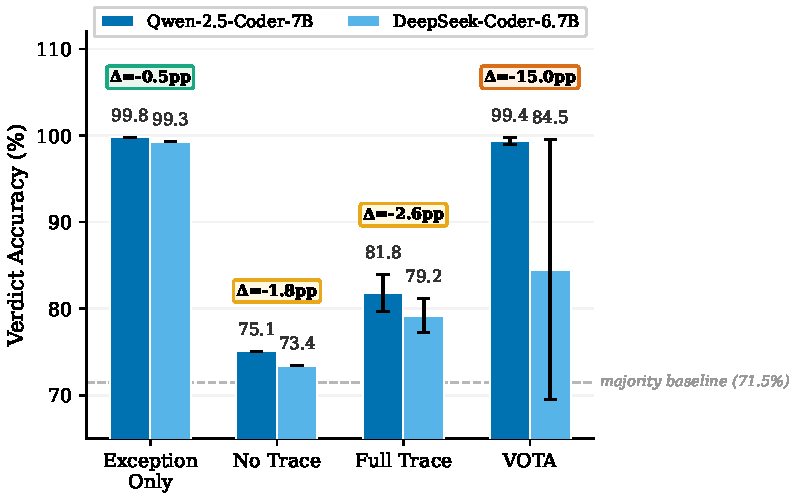
\includegraphics[width=\columnwidth]{fig3_cross_model_gap}
\caption{Cross-model verdict accuracy by trace condition (Qwen-2.5-Coder-7B vs.\ DeepSeek-Coder-6.7B, $N{=}1{,}190$). \cond{exception\_only} shows near-identical accuracy across models ($\Delta{=}0.5$pp), while \cond{VOTA} exhibits a 15pp cross-model gap due to a tokenizer-induced training failure (Appendix~\ref{sec:tokenizer_analysis}).}
\label{fig:cross_scale}
\end{figure}

\section{Related Work}

\subsection{Execution Traces for Code LLMs}

Recent work has scaled trace-augmented training: TracePile \citep{chen2025tracepile} pre-trained on 2.6M execution-annotated samples, while \citet{liu2023codeexecution} pre-trained models to predict execution outputs from traces.
\citet{wang2025dcsh} found trace utility to be task- and format-dependent but did not decompose individual trace components; relative to their work, we contribute a two-tier signal hierarchy, a phase transition in trace-length budgets, calibration analysis, and cross-architecture validation.
NExT \citep{ni2024next} and ET-CoT \citep{eguchi2025etcot} used trace chain-of-thought for execution reasoning, and \citet{ferrando2025execute} found compact traces comparable to full traces, consistent with our density finding.
CRUXEval \citep{gu2024cruxeval}, extended to 19 languages by CRUXEval-X \citep{xu2025cruxevalx}, established execution reasoning benchmarks, though neither decomposes which trace components contribute to \emph{classification} accuracy.
\citet{shi2023distracted} showed LLMs are easily distracted by irrelevant context, providing a complementary explanation for why verbose traces impair SFT learning.
In the prompt compression literature, LLMLingua \citep{jiang2023llmlingua} and Selective Context \citep{li2023selectivecontext} showed that pruning low-information tokens preserves downstream accuracy; TraceCoder \citep{huang2026tracecoder} and InspectCoder \citep{wang2025inspectcoder} apply selective trace extraction for automated debugging; and \citet{haque2025traces} found raw traces provide limited repair benefit.
Our density decomposition complements these methods by quantifying \emph{why} compression helps (gradient dilution explains ${\sim}$24\% of the gap; the remainder reflects inference-time interference).

\subsection{Verdict Prediction and Fault Detection}

Verdict prediction is an instance of the longstanding test oracle problem \citep{barr2015oracle}.
TRACED \citep{ding2024traced} showed execution-aware pretraining improves vulnerability detection; DeepDFA \citep{steenhoek2024deepdfa} and learned program slicing \citep{yadavally2024slicing} combined classical program analysis with deep learning for defect detection.
In patch correctness prediction, representation learning of code changes has progressed from CC2Vec \citep{hoang2020cc2vec} to LLM4PatchCorrect \citep{zhou2024llm4patch} (84.4\%) and APPT \citep{appt2024} (79.7\%); \citet{tian2020patchcorrectness} evaluated change representations for predicting repair correctness.
FuseFL \citep{widyasari2024fusefl} showed that structured fault signals such as stack traces improve localization, and \citet{foster2025mutation} leveraged mutation outcomes to guide test generation; the equivalent-mutant problem \citep{papadakis2019mutation} poses an analogous classification challenge.
Spectrum-based fault localization (SBFL) ranks program elements by suspiciousness from test spectra \citep{abreu2007accuracy,jones2002visualization,wong2014dstar}; recent LLM-based approaches such as AutoFL \citep{kang2024autofl} and AgentFL \citep{qin2024agentfl} share our insight that anomalous execution events carry the strongest diagnostic signal.
In agent-based repair, RepairAgent \citep{bouzenia2025repairagent}, Agentless \citep{xia2024agentless}, SWE-agent \citep{yang2024sweagent}, and OpenHands \citep{wang2025openhands} all incorporate execution feedback in repair workflows; in the SWE-bench ecosystem \citep{jimenez2024swebench}, these agents rely on test verdict signals to guide patch selection, yet which trace components carry that signal most efficiently remains unstudied.
LDB \citep{zhong2024ldb} applies segment-level trace verification for debugging, and SelfDebug \citep{chen2024selfdebug} and Reflexion \citep{shinn2023reflexion} iteratively refine code using execution outcomes.
None of these works isolate individual trace components or compare against rule-based baselines.

\begin{table}[t]
\centering
\caption{Cross-model verdict accuracy (\%, $N{=}1{,}190$) across four models and three architecture families. Bold: best per model. $^\ddag$2-seed mean (seed 42 training failure; Appendix~\ref{sec:tokenizer_analysis}). Multi-seed variance in Appendix~\ref{sec:full_results}.}
\label{tab:cross_model}
\small
\resizebox{\columnwidth}{!}{%
\begin{tabular}{lcccc}
\toprule
\textbf{Condition} & \textbf{Qwen-7B} & \textbf{Qwen-1.5B} & \textbf{CL-13B} & \textbf{DS-6.7B} \\
\midrule
exception\_only & \textbf{99.83} & \textbf{99.83} & \textbf{99.89} & \textbf{99.39} \\
ae\_only & 99.64 & 98.83 & 99.08 & 98.53 \\
VOTA & 99.05 & 99.54 & 98.74 & 99.25$^\ddag$ \\
loop\_only & 86.05 & 79.54 & 77.40 & 80.31 \\
no\_trace & 75.13 & 72.35 & 76.47 & 73.36 \\
\midrule
Majority baseline & \multicolumn{4}{c}{71.51} \\
\bottomrule
\end{tabular}%
}
\end{table}

\subsection{Calibration and Training Dynamics}

Neural network calibration \citep{guo2017calibration}, extended to LLMs \citep{kadavath2022language,geng2024calibration}, studies confidence--correctness alignment; \citet{spiess2025calibration} specifically addressed calibration for code models.
Calibration analysis of trace-based code models remains largely unexplored.
Just-in-time defect prediction \citep{kamei2013large,hoang2019deepjit,pornprasit2021jitline} shares our fault detection motivation but operates on code change features rather than execution traces; our work complements this line by showing that execution-time fault signals can be classified with near-perfect accuracy when properly extracted.
Curriculum learning \citep{bengio2009curriculum}, dataset cartography via training dynamics \citep{swayamdipta2020cartography}, and data selection methods \citep{sachdeva2024dataefficient,xie2023doremi} demonstrate that data quality and ordering improve convergence, consistent with our finding that compact exceptions enable convergence within 50 steps while verbose traces trap the model in oscillation across all 444 training steps.
\citet{yang2024generalization} further showed that fine-tuned LLMs generalize better on concise inputs, providing a complementary perspective on why information density governs SFT effectiveness.


\section{Method}

\subsection{Task Definition}

We study \emph{verdict prediction}: given a Python function, a test input, and an optional execution trace, predict whether the test passes or fails.
The model produces a single token (\textit{pass} or \textit{fail}), making this a binary classification task.
Unlike code generation \citep{chen2025tracepile} or output prediction \citep{gu2024cruxeval}, verdict prediction isolates the model's ability to detect faults from its ability to simulate execution.
The discrete binary outcome makes the effect of each trace component directly measurable, providing cleaner ablation contrasts than generation tasks where output quality varies continuously.

\subsection{Dataset}
\label{sec:dataset}

We sampled 10 candidate solutions per problem from Qwen-2.5-Coder-7B-Instruct (temperature 0.8, top\_p 0.95) for 591 problems from HumanEval \citep{chen2021evaluating} (164) and MBPP-sanitized \citep{austin2021program} (427), executed each against canonical tests with \textit{sys.settrace} to obtain line-level traces and pass/fail verdicts, yielding 5,910 pairs (67\% pass, 33\% fail).
The dataset is split 80/20 by problem ID into 4,720 training and 1,190 test samples (majority baseline: 71.51\%).
The \cond{exception\_only} format collapses passing solutions into identical rows (39.45\% train, 48.99\% test duplicates); these duplicates arise from multiple candidate solutions per problem, with the train--test split enforced at the problem level (472 train / 119 test problems, zero crossover; Appendix~\ref{sec:dedup_stats}).

\subsection{Trace Representations}

We define seven conditions that vary the trace information available:
\begin{itemize}[nosep,leftmargin=1em]
\item \cond{no\_trace}: source code and test input only.
\item \cond{full\_trace}: complete line-by-line trace with variable states.
\item \cond{VOTA}: exception events + assertion-point comparisons + loop compression (Appendix~\ref{sec:vota_algorithm}).
\item \cond{exception\_only}: exception and error events only.
\item \cond{ae\_only}: assertion-point actual/expected pairs only.
\item \cond{loop\_only}: loop compression summaries only.
\item \cond{VOTA\_no\_ae}: VOTA without assertion-point information.
\end{itemize}

\subsection{Models and Training}

We evaluate four models spanning three architecture families: \textbf{Qwen-2.5-Coder-7B/1.5B-Instruct} \citep{qwen2025coder}, \textbf{CodeLlama-13B-Instruct} \citep{roziere2024code}, and \textbf{DeepSeek-Coder-6.7B-Instruct} \citep{deepseek2024coder}, covering a 1.5B--13B parameter range (8.7$\times$).
All conditions use Low-Rank Adaptation (LoRA) \citep{hu2022lora} (rank=16, $\alpha$=32, dropout=0.05) on all linear layers, 3 epochs, effective batch size 32, LR $2 \times 10^{-4}$ with linear warmup/decay, max sequence length 2{,}048 tokens.
Sequences exceeding this limit are truncated while preserving the verdict label.
The primary seed is 42; seeds 123 and 456 test \cond{exception\_only} robustness (Appendix~\ref{sec:training_details}).

\subsection{Loss Ablation}

To disentangle training signal from input signal quality, we introduce \cond{full\_trace\_label\_only}: identical full-trace input but loss computed only on the verdict token (trace positions masked).
Improvement over standard \cond{full\_trace} is attributable to backward-pass signal dilution; the remaining gap to VOTA reflects inference-time input complexity.

\begin{table}[t]
\centering
\caption{Component ablation on Qwen-2.5-7B ($N{=}1{,}190$). Tier~1 signals achieve near-perfect accuracy; combining them (VOTA) slightly dilutes performance. Entries marked $^\dag$/$^\S$/$^\ddag$ are 3-seed mean$\pm$std; per-seed breakdowns in Appendix~\ref{sec:full_results}. Seed $\sigma$ is lowest for \cond{exception\_only} ($\sigma{=}0.00$) and highest for \cond{loop\_only} ($\sigma{=}0.52$); \cond{ae\_only} ($\sigma{=}0.49$) is an outlier, suggesting seed sensitivity tracks input length rather than signal density alone.}
\label{tab:ablation}
\small
\resizebox{\columnwidth}{!}{%
\begin{tabular}{llccc}
\toprule
\textbf{Condition} & \textbf{Components} & \textbf{Acc (\%)} & \textbf{95\% CI} & \textbf{Tier} \\
\midrule
ae\_only & assertion-point & 99.64$^\dag$ & [99.26, 99.87] & 1 \\
exception\_only & exception events & \textbf{99.83} & [99.58, 100.00] & 1 \\
VOTA & exc+ae+loop & 99.05$^\S$ & [98.49, 99.50] & --- \\
VOTA\_no\_ae & exc+loop & 99.41 & [98.90, 99.80] & --- \\
loop\_only & loop compression & 86.05$^\ddag$ & [83.97, 87.96] & 2 \\
full\_trace & complete trace & 81.76 & [79.70, 83.90] & --- \\
no\_trace & none & 75.13 & [72.77, 77.48] & --- \\
\midrule
Regex (best) & exc.\ type regex & 93.61 & --- & --- \\
3-shot (Qwen-7B) & in-context learning & 90.84 & --- & --- \\
Zero-shot (4 models) & prompting & 51.0--93.5 & --- & --- \\
\bottomrule
\end{tabular}%
}
\end{table}

\section{Experiments}

We evaluate two questions:
(1)~Do exception signals generalize across model architectures and scales?
(2)~What is the relative contribution of each trace component?
All experiments use $N{=}1{,}190$ test samples with Wilson 95\% CIs.\footnote{Problem-level split (472/119 problems, zero crossover). Deduplication sensitivity analysis confirms 0.00pp delta across all 19 conditions (Appendix~\ref{sec:dedup_stats}).}
All cross-tier differences are significant at $p{<}.0001$ (paired bootstrap, $B{=}10{,}000$) unless noted.
Under problem-level clustered bootstrap (effective $N{\approx}119$), cross-tier gaps remain significant ($p{<}.001$); within-tier comparisons show partially overlapping CIs.

\subsection{Cross-Model Comparison}
\label{sec:cross_model}

Table~\ref{tab:cross_model} compares four models spanning three architecture families across a 1.5B--13B parameter range.

\paragraph{Exception dominance across families.}
Under \cond{exception\_only}, all four models converge to ${\geq}$99.33\% across all seeds, with a cross-model range of just 0.50pp, the tightest of any condition.
CodeLlama-13B reaches 100\% on one seed; the two persistent errors on Qwen (both \textit{GeneratorExit}; Appendix~\ref{sec:irreducible}) are convergence artifacts rather than hard data limitations.

\paragraph{Scale invariance.}
Exception accuracy is independent of model scale: the smallest model (1.5B) matches the largest (13B) on the same representation (Table~\ref{tab:cross_model}).
In contrast, \cond{no\_trace} scales monotonically with capacity and exhibits the highest seed variance of any condition.
Exception events eliminate both the scale gap and the instability.

\paragraph{VOTA robustness.}
Excluding one training failure caused by tokenizer-induced truncation (Appendix~\ref{sec:tokenizer_analysis}), VOTA achieves ${\geq}$98.57\% across all models within a 0.80pp range.
The failure is itself informative: 91.7\% of that seed's training samples were truncated, while compact \cond{exception\_only} inputs (median 150 tokens) sidestep truncation entirely.

\subsection{Component Ablation}
\label{sec:ablation}

Table~\ref{tab:ablation} decomposes VOTA on Qwen-2.5-7B, revealing a two-tier hierarchy.
Tier~1 signals are individually sufficient: \cond{exception\_only} alone exceeds full VOTA, implying that combining additional components introduces noise rather than value.
Removing assertion points has no effect (\cond{VOTA\_no\_ae}), which reaffirms exception dominance.
The Tier~1/2 boundary is sharp (Figure~\ref{fig:forest_plot}): the weakest Tier~1 condition exceeds the strongest Tier~2 by over 12pp with non-overlapping confidence intervals.
Tier~2 (\cond{loop\_only}) benefits are model-dependent: Qwen-7B gains +10.92pp over \cond{no\_trace} while CodeLlama gains only +0.93pp (n.s.), suggesting loop utilization reflects architectural capacity to exploit structured iteration patterns rather than a universal signal.
Within Tier~2, the larger Qwen-7B outgains Qwen-1.5B (+10.92 vs.\ +7.19pp, $p{<}.0001$), the only condition where scale provides a meaningful advantage.

\paragraph{Baselines.}
The strongest regex heuristic (exception class name matching) trails SFT \cond{exception\_only} by 6.22pp ($p{<}.001$); the gap concentrates on boundary cases where SFT distinguishes caught from uncaught exceptions, correctly resolving 6/8 ambiguous samples vs.\ 0/8 for regex (Appendix~\ref{sec:regex_baselines}).
Zero-shot prompting spans a 42pp range across models; SFT compresses this to 0.50pp with 4,720 training samples (Figure~\ref{fig:zeroshot_vs_sft}; Appendix~\ref{sec:zeroshot_cross_model}).

\begin{table}[t]
\centering
\caption{Information density decomposition on Qwen-7B. Gradient masking (\cond{label\_only}) bounds backward-pass dilution; the remaining gap reflects inference-time input factors. 3-seed means.}
\label{tab:density}
\small
\resizebox{\columnwidth}{!}{%
\begin{tabular}{lccc}
\toprule
\textbf{Condition} & \textbf{Acc (\%)} & \textbf{$\Delta$ vs.\ full\_trace} & \textbf{Gap explained} \\
\midrule
full\_trace & 81.76 & --- & --- \\
label\_only & 85.94{\scriptsize$\pm$1.12} & +4.18pp & 24\% \\
VOTA & 99.05{\scriptsize$\pm$0.38} & +17.29pp & 100\% \\
\bottomrule
\end{tabular}%
}
\end{table}

\subsection{Format Marker Ablation}
\label{sec:nomarker}

The \cond{exception\_only} format includes a ``[No exception data in trace]'' marker for pass-class samples.
Retraining with all format markers removed (\cond{nomarker}) yields a modest drop (${\sim}$2pp on both Qwen-7B and Qwen-1.5B), accounting for only ${\sim}$9\% of the total exception lift over \cond{no\_trace}.
Exception events thus provide two signal layers: structural markers (${\sim}$2pp, regex-learnable) and semantic content (${\sim}$22pp, requiring SFT to distinguish caught from uncaught exceptions).
Both layers show no degradation at smaller scale.

\begin{figure}[t]
\centering
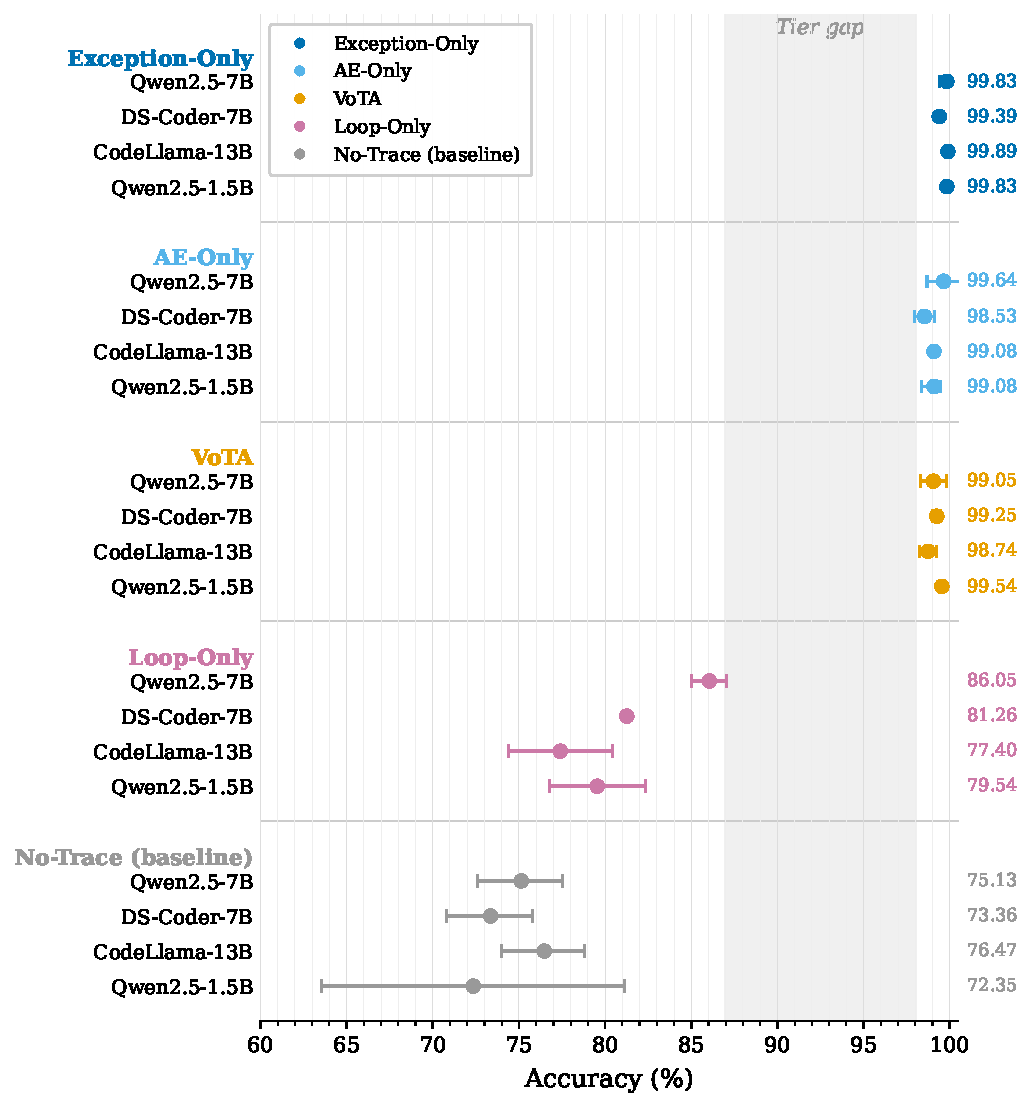
\includegraphics[width=\columnwidth]{forest_plot_tier_boundary}
\caption{Cross-model accuracy with 95\% Wilson CIs across all conditions and four models. The shaded region highlights the Tier~1/2 boundary gap ({>}12pp). Within Tier~1, all models converge to $\geq$99.08\%; within Tier~2, performance is model-dependent.}
\label{fig:forest_plot}
\end{figure}

\begin{figure*}[t]
\centering
\begin{minipage}[t]{0.48\textwidth}
\centering
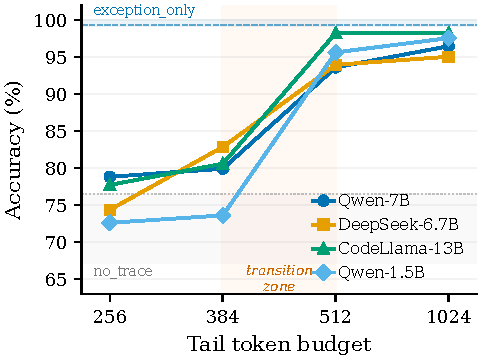
\includegraphics[width=\textwidth]{budget_curve}
\end{minipage}\hfill
\begin{minipage}[t]{0.48\textwidth}
\centering
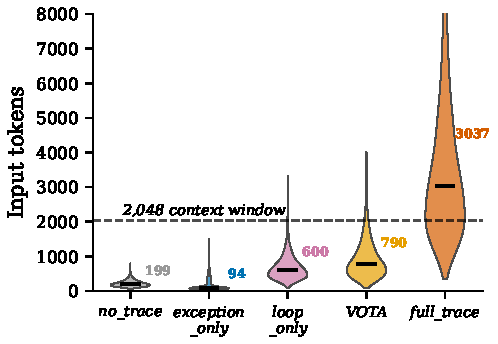
\includegraphics[width=\textwidth]{token_distribution}
\end{minipage}
\caption{(\textbf{Left}) Cross-model tail-truncation budget curve ($N{=}1{,}190$, four models). All models remain near baseline at tail-256/384, then jump sharply at 384$\to$512 as the exception traceback is captured (shaded). Dashed: \cond{exception\_only} range; dotted: \cond{no\_trace} range. (\textbf{Right}) Input token length distribution across trace conditions (training set, $N{=}4{,}720$). Dashed line: 2,048-token context window. \cond{exception\_only} inputs (median 150 tokens) fit entirely within the window, while \cond{full\_trace} inputs frequently exceed it, triggering truncation.}
\label{fig:trace_length}
\label{fig:token_distribution}
\end{figure*}

\subsection{Information Density Decomposition}
\label{sec:density}

The gap between \cond{full\_trace} and VOTA decomposes via \cond{full\_trace\_label\_only}, which retains the full trace input but masks all trace tokens from the loss (Table~\ref{tab:density}).

Gradient masking places an upper bound on backward-pass dilution: the +4.18pp gain bounds the backward-pass contribution to ${\sim}$24\% of the full gap.
The remaining majority of the gap persists even with identical loss computation, suggesting that interference from thousands of irrelevant trace lines at inference, rather than training signal dilution, is the dominant factor.
Cross-model evidence corroborates this: the tail-truncation phase transition at ${\sim}$500 tokens (\S\ref{sec:trace_length}) coincides with exception traceback length, and cross-scale validation on Qwen-1.5B yields a consistent pattern (gradient masking explains a similar minority share).
CodeLlama and DeepSeek exhibit label-only collapse, limiting the decomposition to models whose tokenizers preserve sufficient trace structure.
Error analysis confirms all \cond{full\_trace} errors occur where truncation removes diagnostic markers (Figure~\ref{fig:token_distribution}).
The two factors may interact, and the decomposition is approximate (Qwen family, 2 scales, 3 seeds).

\subsection{Additional Analyses}
\label{sec:additional}

\paragraph{Tail-truncation budget curve.}
\label{sec:trace_length}
A cross-model budget sweep reveals a sharp phase transition between 384 and 512 tail tokens (Figure~\ref{fig:trace_length}).
Below this threshold, all models remain near baseline regardless of how many tokens are retained.
Above it, accuracy jumps by 13--22pp in a single step, converging into a narrow band by tail-1024.
The transition zone coincides with the typical exception traceback length (${\sim}$400--500 tokens), providing spatial evidence that diagnostic events in the trace tail drive the accuracy gains.

Tail-truncation dramatically outperforms head-truncation: retaining the last $k$ tokens exceeds retaining the first $k$ by 15--23pp across models.
Under head-truncation, accuracy is non-monotonic and confined to a narrow band, because mid-length prefixes retain enough irrelevant content to mislead the model while discarding diagnostic events near the trace terminus (Appendix~\ref{sec:trace_length_full}).

\paragraph{Calibration.}
\label{sec:calibration}
Calibration mirrors the tier hierarchy: \cond{exception\_only} achieves an Expected Calibration Error (ECE) of 0.003 vs.\ 0.171 for \cond{no\_trace}, a 63$\times$ gap (Figure~\ref{fig:calibration}).
This advantage generalizes across all four models (ECE~${<}$~0.007; Appendix~\ref{sec:calibration_full}).

\paragraph{Error orthogonality and exception types.}
\cond{exception\_only}'s residual errors have zero overlap with all other conditions' error sets (Jaccard\,=\,0.000; Figure~\ref{fig:error_overlap}), which confirms it operates on an independent signal dimension.
All standard exception types achieve 100\% accuracy; the only failures arise from \textit{GeneratorExit}, a benign \textit{BaseException} subclass (Appendix~\ref{sec:exception_type}).

\paragraph{Cross-dataset generalization.}
\label{sec:debugbench}
DebugBench \citep{tian2024debugbench} ($N{=}426$) preserves the component ranking (\cond{exception\_only} 100\%, VOTA 99.77\%, \cond{no\_trace} 96.71\%), though narrow margins reflect a ceiling effect from structurally distinctive mutations (Appendix~\ref{sec:debugbench_full}).


\section{Discussion}

\begin{figure}[t]
\centering
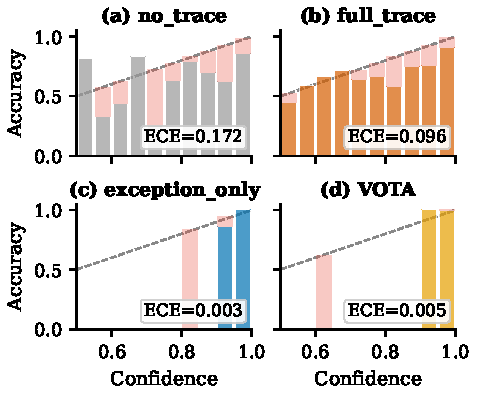
\includegraphics[width=\columnwidth]{fig2_calibration}
\caption{Reliability diagrams for four trace conditions on Qwen-2.5-7B ($N{=}1{,}190$). \cond{exception\_only} (ECE=0.003) clusters near the diagonal; \cond{no\_trace} (ECE=0.171) shows systematic overconfidence.}
\label{fig:calibration}
\end{figure}

The central finding is that information density governs learning efficiency for trace-based verdict prediction.
Exception events concentrate the fault signal in a compact format (median 150 tokens), while non-exception components record \emph{how} the program ran, not \emph{whether} it failed.
This explains three patterns: (1)~adding information beyond exceptions provides no benefit (indeed, VOTA underperforms \cond{exception\_only}, Table~\ref{tab:ablation}); (2)~the tail-truncation phase transition at ${\sim}$500 tokens coincides with the diagnostic-event boundary (Figure~\ref{fig:trace_length}); and (3)~the SFT advantage over regex concentrates on caught-exception boundary cases (\S\ref{sec:nomarker}).
The narrow cross-model gap (Table~\ref{tab:cross_model}) supports density, not capacity, as the binding constraint.

\paragraph{SFT vs.\ regex: semantic understanding.}
Format-marker removal drops accuracy by only ${\sim}$2pp, leaving a clear gap over the best regex.
On boundary samples with caught exceptions, SFT correctly classifies 6/8 vs.\ 0/8 for regex ($p{=}.041$). This confirms the signal is semantic rather than syntactic.
This distinction matters for deployment: regex baselines can detect most exceptions through surface-level pattern matching, but fail precisely on the ambiguous cases (caught exceptions within \textit{try/except} blocks) where correct classification requires understanding the exception's role in program control flow.
SFT learns this distinction from fewer than 5{,}000 training examples, suggesting that the relevant semantic features are readily extractable from pretrained code representations when the input is sufficiently compact.

\paragraph{Near-perfect floor.}
The two residual errors (both \textit{GeneratorExit}; Appendix~\ref{sec:error_overlap}) are shared across configurations and models.
One seed achieves 100\%, which establishes 99.83\% as a convergence \emph{floor}, not a ceiling.
The error overlap analysis (Figure~\ref{fig:error_overlap}) reveals that these errors are orthogonal to all other conditions' error sets (Jaccard = 0.000); \cond{exception\_only} therefore operates on an independent signal dimension.
The practical implication is that the two residual errors cannot be resolved by adding more trace information; they require disambiguating benign \textit{BaseException} subclasses from genuine faults, a representation-level fix rather than a data quantity issue.

\begin{figure}[t]
\centering
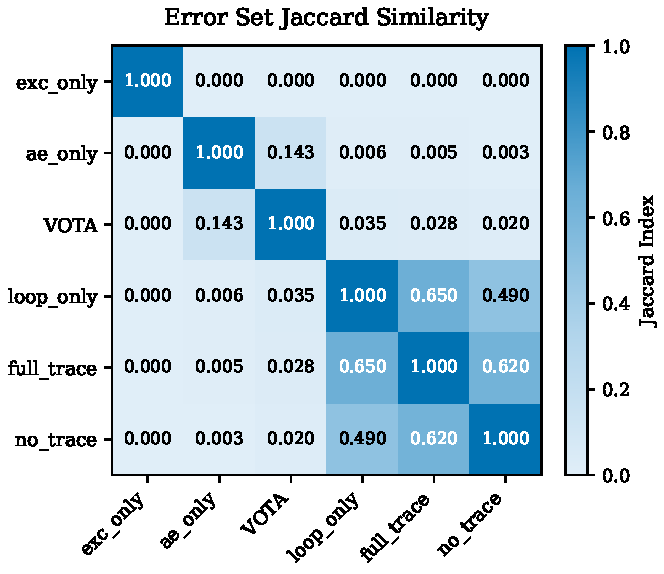
\includegraphics[width=\columnwidth]{error_overlap}
\caption{Pairwise Jaccard similarity between error sets (Qwen-7B, $N{=}1{,}190$). \cond{exception\_only} has zero overlap with all other conditions and operates on an independent signal dimension.}
\label{fig:error_overlap}
\end{figure}

\paragraph{Tier hierarchy and design principles.}
The two-tier structure (Figure~\ref{fig:forest_plot}) suggests a hierarchical extraction strategy: extract exception events first, resort to Tier~2 signals only when no exception is raised.
Within Tier~1, both \cond{exception\_only} and \cond{ae\_only} achieve near-perfect accuracy independently, yet combining them in VOTA slightly \emph{degrades} performance, a counter-intuitive finding that underscores how additional signal can introduce noise when the primary signal is already sufficient.
Loop benefit is model-dependent (Qwen-7B gains +10.92pp while CodeLlama gains only +0.93pp). This reflects an architecture-level capacity to exploit structured iteration patterns rather than a universal signal.
This density--efficiency link should transfer to any trace-based task where compact diagnostic events exist within verbose runtime logs, such as crash triage in continuous integration, where stack traces carry far more signal than full execution histories.

\paragraph{Cross-model robustness and scale independence.}
The cross-model analysis reveals that \cond{exception\_only}'s accuracy range is ${<}$1pp across four models (1.5B--13B) vs.\ ${\sim}$9pp for \cond{loop\_only}, demonstrating that compact inputs eliminate the architecture-dependent variance that plagues verbose representations.
This scale independence is striking: the smallest model (Qwen-1.5B at 1.5B parameters) matches the largest (CodeLlama-13B at 13B parameters) when given the same compact input, whereas \cond{no\_trace} accuracy scales monotonically with model capacity (Table~\ref{tab:cross_model}).
The zero-shot comparison reinforces this: SFT compresses a 42.44pp cross-architecture range to just 0.50pp with only 4{,}720 training samples (Figure~\ref{fig:zeroshot_vs_sft}), making exception-based verdict prediction accessible to smaller models without sacrificing accuracy.
Label-only loss on high-truncation tokenizers causes model collapse, further confirming density as the binding constraint: when the tokenizer is inefficient, even masking trace tokens from the loss cannot compensate for the inference-time interference from thousands of irrelevant tokens.

\begin{figure}[t]
\centering
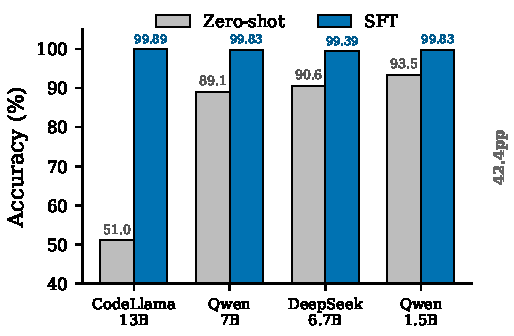
\includegraphics[width=\columnwidth]{zeroshot_vs_sft}
\caption{Zero-shot vs.\ SFT \cond{exception\_only} accuracy across four models ($N{=}1{,}190$). SFT compresses the cross-architecture variance from 42.44pp to 0.50pp.}
\label{fig:zeroshot_vs_sft}
\end{figure}

\paragraph{Exception events capture test verdicts, not just crashes.}
A natural concern is that exception-based classification merely detects program crashes.
In fact, 55.5\% of failures in our dataset are silent logic errors where the program terminates normally but produces incorrect output.
\cond{exception\_only} nonetheless achieves 100\% fail recall because test assertions generate \textit{AssertionError} events that explicitly mark the discrepancy between actual and expected behavior.
This means the ``exception'' signal subsumes both crash-type and assertion-type failures, making it a complete verdict signal rather than a crash detector.

\paragraph{Alternative explanations.}
Three alternatives merit discussion.
\emph{Length asymmetry}: padding all inputs to the maximum sequence length leaves accuracy unchanged, ruling out a confound from batch-level length variation.
\emph{Format-marker familiarity}: removing markers accounts for only ${\sim}$9\% of the exception lift, though familiarity with exception formats in pretraining data cannot be fully controlled for.
\emph{Positional concentration}: diagnostic information concentrates in the trace tail (\S\ref{sec:trace_length}); the tail-truncation budget curve localizes the critical threshold to ${\sim}$400--500 tokens, consistent with typical exception traceback length, but fully disentangling positional proximity from semantic density requires future work with controlled position-shuffled experiments.

\paragraph{Connections to prompt compression.}
Our findings align with the prompt compression literature: LLMLingua \citep{jiang2023llmlingua} and Selective Context \citep{li2023selectivecontext} showed that pruning low-information tokens preserves downstream accuracy.
The trace domain provides a natural instance of this phenomenon: exception events are effectively a domain-specific compression that retains the diagnostic tokens and discards the execution log.
The information density decomposition (\S\ref{sec:density}) quantifies this: removing all non-diagnostic tokens accounts for the majority of the performance gap, while backward-pass gradient dilution explains at most 24\%.

\paragraph{Learning dynamics.}
\cond{exception\_only} converges within 50 steps and saturates by step 150, while \cond{full\_trace} oscillates across all 444 training steps without reaching stable convergence (Figure~\ref{fig:training_dynamics}).
Seed variance negatively correlates with input density (Table~\ref{tab:ablation}): \cond{exception\_only} shows zero cross-seed variance ($\sigma{=}$0.00) while \cond{loop\_only} exhibits the highest ($\sigma{=}$0.52).
This pattern suggests that compact inputs not only improve final accuracy but also stabilize the optimization landscape, reducing sensitivity to random initialization.
From a practical standpoint, this means exception-based models can be trained with a single seed and minimal hyperparameter tuning, whereas verbose-trace models require multiple seeds and careful early-stopping selection.

\begin{figure}[t]
\centering
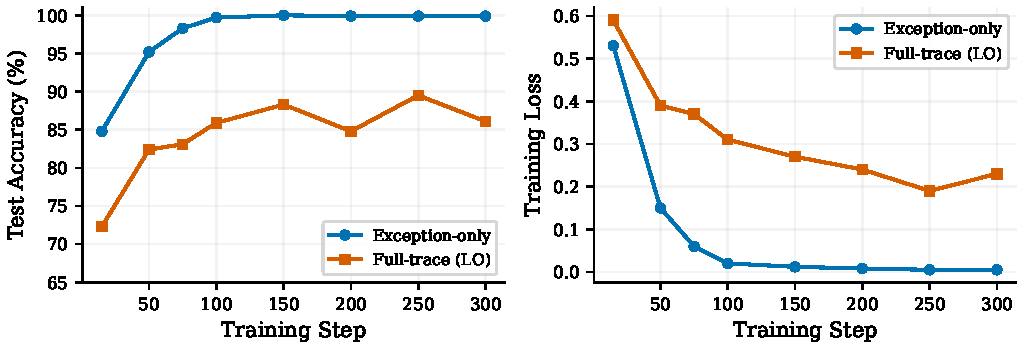
\includegraphics[width=\columnwidth]{training_dynamics}
\caption{Training dynamics comparison. \cond{exception\_only} (blue) converges within 50 steps and saturates by step 150. \cond{full\_trace} with label-only loss (red, dashed) oscillates without stable convergence across all 444 training steps.}
\label{fig:training_dynamics}
\end{figure}

\section{Conclusion}

We presented the first systematic component ablation of trace representations for verdict prediction, covering four code models across three architecture families.
The finding is clear: information density, not trace completeness, determines learning efficiency under SFT.
Compact exception events converge to ${\geq}$99.33\% across all models, while verbose full traces oscillate without stable convergence.
These results establish a two-tier diagnostic hierarchy: Tier~1 signals (exceptions, assertion comparisons) generalize across architectures within a 0.50--1.11pp range, while Tier~2 signals (loop patterns) are model-dependent. For structurally constrained tasks such as verdict prediction, targeted signal extraction should replace wholesale trace inclusion.


\section*{Limitations}

Our study has three main limitations.
First, all experiments use Python execution traces from code-specialized models ranging from 1.5B to 13B parameters; whether the observed density--efficiency relationship holds for other programming languages, human-written code, or larger models (30B+) remains untested.
Second, our findings may not generalize beyond the current setting: Python's structured exception hierarchy makes exception events particularly informative, and languages with less structured error reporting may exhibit different signal distributions.
Third, the gradient masking experiment isolates backward-pass signal dilution but does not quantify forward-pass attention effects; disentangling these two factors requires further investigation.

\bibliography{references}

\clearpage
\appendix
\makeatletter
\renewcommand{\verbatim@font}{\normalfont\rmfamily\small}
\makeatother
\section{Per-Class Performance Breakdown}
\label{sec:per_class}

Table~\ref{tab:per_class} reports per-class precision, recall, and F1 for all experimental conditions.

\begin{table*}[t]
\centering
\caption{Per-class precision, recall, and F1 for all experimental conditions (seed 42). DeepSeek VOTA seed 42 is a training failure (84.45\%, fail recall = 45.4\%) due to tokenizer-driven truncation; seeds 123/456 achieve 99.16\%/99.33\%.}
\label{tab:per_class}
\small
\begin{tabular}{llccccccc}
\toprule
\textbf{Condition} & \textbf{Model} & \textbf{Acc} & \textbf{Pass P} & \textbf{Pass R} & \textbf{Pass F1} & \textbf{Fail P} & \textbf{Fail R} & \textbf{Fail F1} \\
\midrule
No Trace          & Qwen-2.5-7B & 75.13 & 87.76 & 75.79 & 81.34 & 54.73 & 73.45 & 62.72 \\
Full Trace        & Qwen-2.5-7B & 81.76 & 87.74 & 86.60 & 87.17 & 67.43 & 69.62 & 68.51 \\
Full Trace (LO)   & Qwen-2.5-7B & 85.94 & 88.21 & 93.18 & 90.63 & 80.07 & 68.73 & 73.97 \\
VOTA              & Qwen-2.5-7B & 99.05 & 100.00 & 99.18 & 99.59 & 97.98 & 100.00 & 98.98 \\
Exception Only    & Qwen-2.5-7B & 99.83 & 100.00 & 99.76 & 99.88 & 99.41 & 100.00 & 99.71 \\
AE Only           & Qwen-2.5-7B & 99.92 & 100.00 & 99.88 & 99.94 & 99.71 & 100.00 & 99.85 \\
Loop Only         & Qwen-2.5-7B & 86.05 & 92.39 & 87.07 & 89.66 & 71.65 & 82.01 & 76.48 \\
VOTA\_no\_ae       & Qwen-2.5-7B & 99.41 & 99.88 & 99.29 & 99.59 & 98.26 & 99.71 & 98.98 \\
\midrule
No Trace          & DeepSeek-6.7B & 73.36 & 81.71 & 80.85 & 81.28 & 53.16 & 54.57 & 53.86 \\
Full Trace        & DeepSeek-6.7B & 79.16 & 85.70 & 85.10 & 85.40 & 63.20 & 64.30 & 63.70 \\
VOTA              & DeepSeek-6.7B & 84.45 & 82.14 & 100.00 & 90.20 & 100.00 & 45.40 & 62.50 \\
Exception Only    & DeepSeek-6.7B & 99.33 & 100.00 & 99.06 & 99.53 & 97.69 & 100.00 & 98.83 \\
AE Only           & DeepSeek-6.7B & 98.74 & 98.40 & 99.90 & 99.10 & 99.70 & 95.90 & 97.70 \\
\bottomrule
\end{tabular}
\end{table*}

%% ============================================================
\section{Training Details}
\label{sec:training_details}

Table~\ref{tab:hyperparams} summarizes the training hyperparameters shared across all conditions.
All experiments use the HuggingFace TRL \textit{SFTTrainer} with LoRA \citep{hu2022lora} applied to all linear layers.

\begin{table}[h!]
\centering
\caption{Training hyperparameters (shared across all conditions).}
\label{tab:hyperparams}
\small
\resizebox{\columnwidth}{!}{%
\begin{tabular}{ll}
\toprule
\textbf{Hyperparameter} & \textbf{Value} \\
\midrule
LoRA rank ($r$)            & 16 \\
LoRA alpha ($\alpha$)      & 32 \\
LoRA dropout               & 0.05 \\
LoRA target modules        & all linear layers \\
\midrule
Epochs                     & 3 \\
Per-device batch size       & 4 \\
Gradient accumulation steps & 8 \\
Effective batch size        & 32 \\
\midrule
Learning rate               & $2 \times 10^{-4}$ \\
LR scheduler                & linear decay \\
Warmup ratio                & 0.1 \\
Weight decay                & 0.01 \\
\midrule
Max sequence length         & 2048 tokens \\
Primary seed                & 42 \\
Robustness seeds            & 123, 456 \\
\midrule
Hardware                    & 1$\times$ RTX PRO 6000 Blackwell (96\,GB VRAM) \\
Framework                   & HuggingFace TRL SFTTrainer \\
\bottomrule
\end{tabular}%
}
\end{table}

Table~\ref{tab:train_time} reports per-condition training wall-clock times.
Conditions with longer trace inputs (e.g., \textit{full\_trace}, VOTA) require proportionally more training time due to increased sequence lengths.

\begin{table}[h!]
\centering
\caption{Training wall-clock time per condition on a single RTX PRO 6000 Blackwell GPU. Where multiple seeds were run, individual times are listed.}
\label{tab:train_time}
\small
\begin{tabular}{llr}
\toprule
\textbf{Condition} & \textbf{Seed(s)} & \textbf{Time (h)} \\
\midrule
no\_trace       & 42         & ${\sim}$0.5 \\
full\_trace     & 42         & ${\sim}$2.2 \\
label\_only     & 42         & ${\sim}$2.2 \\
VOTA                     & 42         & ${\sim}$2.3 \\
exception\_only & 42         & ${\sim}$2.1 \\
exception\_only & 123        & ${\sim}$2.1 \\
exception\_only & 456        & ${\sim}$1.3 \\
ae\_only        & 42         & ${\sim}$1.8 \\
loop\_only      & 42         & ${\sim}$2.1 \\
VOTA\_no\_ae    & 42         & ${\sim}$1.8 \\
\bottomrule
\end{tabular}
\end{table}

%% ============================================================
\section{VOTA Extraction Algorithm}
\label{sec:vota_algorithm}

Algorithm~\ref{alg:vota} describes the three-component VOTA extraction pipeline applied to a raw \textit{sys.settrace} execution log.

\begin{algorithm}[h!]
\caption{VOTA Trace Extraction}
\label{alg:vota}
\small
\begin{algorithmic}[1]
\REQUIRE Raw trace $T$ from \textit{sys.settrace} (list of events)
\ENSURE Compressed VOTA representation $V$
\STATE $V \leftarrow$ empty string
\STATE \textbf{// Component 1: Exception summary}
\FOR{each event $e$ in $T$ with type \textit{exception}}
  \STATE Parse traceback $\rightarrow$ extract error type, message, file, line
  \STATE Append \textit{[ERROR] type: message (file:line)} to $V$
\ENDFOR
\IF{no exception events found}
  \STATE Append \textit{[No exception data in trace]} to $V$
\ENDIF
\STATE \textbf{// Component 2: Assertion-point comparison}
\FOR{each \textit{assert} or \textit{return} event $e$ in $T$}
  \STATE Extract actual value from execution state
  \STATE Extract expected value from test assertion
  \STATE Append \textit{[ASSERT] actual=... expected=... match=T/F} to $V$
\ENDFOR
\STATE \textbf{// Component 3: Loop compression}
\FOR{each consecutive repeated line sequence $S$ in $T$}
  \IF{$|S| \geq 2$ iterations of same loop body}
    \STATE Replace $S$ with single iteration + \textit{[repeated $\times$N]}
  \ENDIF
\ENDFOR
\STATE Append compressed non-exception lines to $V$
\RETURN $V$
\end{algorithmic}
\end{algorithm}

%% ============================================================
\section{VOTA Trace Examples}
\label{sec:vota_examples}

We provide two representative VOTA trace examples illustrating the fail and pass cases.
In the fail case, the exception event provides an unambiguous fault signal.
In the pass case, the absence of an exception event combined with a matching assertion point confirms correct execution.

\paragraph{Fail example.}
A \textit{ZeroDivisionError} triggers an \textit{[ERROR]} event, providing a direct fault signal that is sufficient for the model to predict \textit{fail}.

\begin{scriptsize}
\begin{verbatim}
## Function
def divide(a, b):
    return a / b

## Test Input
divide(1, 0)

## Expected Output
inf

## VOTA Trace
[ERROR] ZeroDivisionError: division by zero

## Verdict
fail
\end{verbatim}
\end{scriptsize}

\paragraph{Pass example.}
No exception is raised, and the assertion point confirms that the actual output matches the expected value.

\begin{scriptsize}
\begin{verbatim}
## Function
def add(a, b):
    return a + b

## Test Input
add(2, 3)

## Expected Output
5

## VOTA Trace
[LOOP] No loops detected.
[ASSERT] actual=5, expected=5

## Verdict
pass
\end{verbatim}
\end{scriptsize}

These examples illustrate the core asymmetry exploited by the \textit{exception\_only} condition: fail cases produce an explicit \textit{[ERROR]} event, while pass cases are characterized by its absence.
This binary signal (presence vs.\ absence of an exception) is sufficient for near-perfect verdict prediction.

%% ============================================================
\section{Full Experimental Results}
\label{sec:full_results}

Table~\ref{tab:cross_model} reports seed 42 (primary seed) results for all conditions.
Table~\ref{tab:cross_model_multiseed} extends this with multi-seed means and standard deviations where robustness seeds were run.

\paragraph{Seeding strategy.}
All conditions were run with seed 42 as the primary seed.
Robustness seeds (123, 456) were added for conditions central to the paper's claims: \textit{exception\_only} and VOTA across all four models, and the full ablation set (ae\_only, loop\_only, label\_only) on Qwen-7B.
Baseline conditions (\textit{no\_trace}, \textit{full\_trace}) were run with a single seed because they serve as reference points whose absolute values matter less than the gap to Tier~1 conditions; where multi-seed baselines were run (Qwen-1.5B \textit{no\_trace}, 3 seeds), the high variance ($\pm$4.48pp) further confirms instability relative to \textit{exception\_only}'s zero variance.
Conditions specific to a single analysis (\textit{VOTA\_no\_ae}, gradient masking) were run with a single seed to conserve compute.

\begin{table}[h!]
\centering
\caption{Cross-model multi-seed results (\%, $N{=}1{,}190$). Mean$\pm$std across available seeds; entries without $\pm$ are single-seed. $^\ddag$2-seed mean (seed 42 training failure excluded; \S\ref{sec:tokenizer_analysis}).}
\label{tab:cross_model_multiseed}
\small
\resizebox{\columnwidth}{!}{%
\begin{tabular}{lcccc}
\toprule
\textbf{Condition} & \textbf{Qwen-7B} & \textbf{Qwen-1.5B} & \textbf{CL-13B} & \textbf{DS-6.7B} \\
\midrule
exception\_only & 99.83{\scriptsize$\pm$0.00} & 99.83{\scriptsize$\pm$0.00} & 99.89{\scriptsize$\pm$0.10} & 99.39{\scriptsize$\pm$0.10} \\
ae\_only & 99.64{\scriptsize$\pm$0.49} & 98.83{\scriptsize$\pm$0.36} & 99.08{\scriptsize$\pm$0.00} & 98.53{\scriptsize$\pm$0.30} \\
VOTA & 99.05{\scriptsize$\pm$0.38} & 99.54{\scriptsize$\pm$0.06} & 98.74{\scriptsize$\pm$0.24} & 99.25$^\ddag$ \\
loop\_only & 86.05{\scriptsize$\pm$0.52} & 79.54{\scriptsize$\pm$1.42} & 77.40{\scriptsize$\pm$1.54} & 80.31{\scriptsize$\pm$1.65} \\
no\_trace & 75.13 & 72.35{\scriptsize$\pm$4.48} & 76.47 & 73.36 \\
\midrule
Majority baseline & \multicolumn{4}{c}{71.51} \\
\bottomrule
\end{tabular}%
}
\end{table}

Tables~\ref{tab:full_qwen} and \ref{tab:full_deepseek} report the complete per-seed results for Qwen-7B and DeepSeek-6.7B.

\begin{table}[h!]
\centering
\caption{Full results for Qwen-2.5-Coder-7B across all conditions and seeds. Conditions with a single seed report no variance. \textit{exception\_only} achieves 99.83\% across all three seeds ($\sigma{=}$0). \textit{ae\_only} achieves 99.64\% mean ($\pm$0.49; seed 123 at 99.08\% is the outlier).}
\label{tab:full_qwen}
\small
\resizebox{\columnwidth}{!}{%
\begin{tabular}{lcccc}
\toprule
\textbf{Condition} & \textbf{S42} & \textbf{S123} & \textbf{S456} & \textbf{Mean $\pm$ Std} \\
\midrule
exception\_only & 99.83 & 99.83 & 99.83 & 99.83 $\pm$ 0.00 \\
ae\_only        & 99.92 & 99.08 & 99.92 & 99.64 $\pm$ 0.49 \\
VOTA                     & 99.41 & 98.66 & 99.08 & 99.05 $\pm$ 0.38 \\
VOTA\_no\_ae    & 99.41 & ---   & ---   & --- \\
label\_only     & 86.22 & 86.89 & 84.70 & 85.94 $\pm$ 1.12 \\
loop\_only      & 85.63 & 85.88 & 86.64 & 86.05 $\pm$ 0.52 \\
full\_trace     & 81.76 & ---   & ---   & --- \\
no\_trace       & 75.13 & ---   & ---   & --- \\
\bottomrule
\end{tabular}%
}
\end{table}

\begin{table}[h!]
\centering
\caption{Full results for DeepSeek-Coder-6.7B across all conditions and seeds. \textit{exception\_only} is consistent across seeds: 99.33/99.50/99.33 ($\sigma{=}$0.10pp).}
\label{tab:full_deepseek}
\small
\resizebox{\columnwidth}{!}{%
\begin{tabular}{llcc}
\toprule
\textbf{Condition} & \textbf{Seed} & \textbf{Accuracy} & \textbf{Notes} \\
\midrule
exception\_only & 42  & 99.33 & epoch 1: 99.83 \\
exception\_only & 456 & 99.33 & CI [98.82, 99.75] \\
exception\_only & 123 & 99.50 & \\
\midrule
VOTA                     & 42  & 84.45 & training failure; fail recall = 45.4\% \\
VOTA                     & 123 & 99.16 & \\
VOTA                     & 456 & 99.33 & \\
no\_trace       & 42  & 73.36 & \\
full\_trace     & 42  & 79.16 & CI [76.80, 81.30] \\
\bottomrule
\end{tabular}%
}
\end{table}

%% ============================================================
\section{Tokenizer and Truncation Analysis}
\label{sec:tokenizer_analysis}

DeepSeek VOTA seed 42 (84.45\%) is a training failure driven by tokenizer-induced truncation.
Re-evaluation of the seed 42 checkpoint with the standard max\_length=2048 yields 16\% accuracy, which confirms complete model collapse rather than marginal degradation.
The previously reported 84.45\% was obtained with max\_length=16384, which partially bypasses tokenizer truncation.
Seeds 123 and 456, evaluated under identical conditions, achieve 99.16\% and 99.33\% respectively.
The DeepSeek tokenizer averages 2{,}626 tokens per VOTA sample versus 1{,}929 for Qwen, causing 91.7\% of DeepSeek VOTA training samples to exceed the 2{,}048-token context window.
The training framework preserves the verdict label but truncates trace content, so the model trains with incomplete diagnostic information for the majority of samples.
Seeds 123 and 456 (99.16\% and 99.33\%) demonstrate that DeepSeek can learn VOTA when LoRA initialization avoids the truncation-sensitive basin; the 2-seed mean (99.25\%$\pm$0.12) matches the cross-model VOTA range (98.74--99.54\%).

A post-hoc group analysis on seed 42 provides directional evidence: partitioning test samples by whether their training-set counterparts exceeded the context window, intact samples ($N{=}99$) achieve 100\% accuracy while truncated samples ($N{=}1{,}091$) achieve 83.04\% (95\% CI [80.75\%, 85.24\%]; Fisher exact $p{<}.001$), with all 185 errors concentrated in the fail class (fail recall = 31.23\%).
Per-class analysis (Table~\ref{tab:per_class}) confirms that seed 42 achieves 100\% fail precision but only 45.43\% fail recall, systematically defaulting to \textit{pass}.

Seed robustness is consistent across models: Qwen \textit{exception\_only} produces identical 99.83\% across all three seeds ($\sigma{=}0$), and DeepSeek achieves 99.39\%$\pm$0.10 (seeds 42/456: 99.33\%, seed 123: 99.50\%).
Because \textit{exception\_only} test inputs contain 48.99\% duplicates (607 unique of 1,190; \S\ref{sec:dataset}), CIs assume $n{=}1{,}190$ independent trials; under deduplication ($n{=}607$), Qwen's accuracy is 99.67\% (Wilson CI [98.81, 99.91]).

%% ============================================================
\section{Irreducible Sample Analysis}
\label{sec:irreducible}

The \textit{exception\_only} condition with Qwen-2.5-Coder-7B misclassifies exactly 2 out of 1,190 test samples across all three seeds (42, 123, 456), with 100\% overlap across seeds.
Both samples (IDs 901 and 905) share the following characteristics:

\begin{itemize}
\item \textbf{Function:} \textit{check\_dict\_case} (HumanEval/95), a function that checks whether all dictionary keys are uniformly upper-case or lower-case strings.
\item \textbf{Ground-truth label:} \textit{pass}.
\item \textbf{Predicted label:} \textit{fail} (false negative).
\item \textbf{Cross-seed consistency:} Both samples are misclassified identically by all three seeds, which indicates a systematic rather than stochastic error.
\end{itemize}

Manual inspection reveals the root cause: \textit{check\_dict\_case} uses \textit{all()} over a generator expression, and Python's \textit{all()} short-circuits on the first \textit{True} value, raising \textit{GeneratorExit} to terminate the generator.
Because \textit{GeneratorExit} is a \textit{BaseException} subclass, the tracer records it as seven \textit{[ERROR] GeneratorExit} lines, even though the function executes correctly and the test passes.
The model observes these spurious error markers and reasonably but incorrectly predicts \textit{fail}.
This is not a model failure but a representation ambiguity: the \textit{exception\_only} format cannot distinguish genuine exceptions from benign \textit{BaseException} subclasses triggered by Python's iterator protocol.

Most configurations converge to these same 2 errors: Qwen-1.5B, Qwen-7B (3 seeds), CodeLlama-13B (seeds 42/456), and DeepSeek-6.7B (seeds 42/456) all produce error set $\{901, 905\}$.
However, CodeLlama-13B seed 123 achieves 100\% accuracy (0/1190 errors), correctly classifying both samples.
This demonstrates that 99.83\% is a near-perfect \emph{floor} (the convergence attractor for most LoRA initializations) rather than a hard data ceiling: the representation supports perfect accuracy, but most initializations converge to the same 2-error basin.
The practical implication is that these errors are high-probability convergence artifacts addressable through seed selection or ensemble methods, not fundamental limitations of the exception-based representation.

%% ============================================================
\section{Exception Type Accuracy Breakdown}
\label{sec:exception_type}

Table~\ref{tab:exception_type} reports \textit{exception\_only} accuracy stratified by exception type on Qwen-2.5-7B (seed=42, $N{=}1{,}190$).
All standard exception types (\textit{TypeError}, \textit{ValueError}, \textit{IndexError}, etc.) achieve 100\% accuracy.
The only misclassifications arise from \textit{GeneratorExit}, a \textit{BaseException} subclass that is not an \textit{Exception}. It is raised by Python's iterator protocol during generator short-circuiting, not by actual program errors.

\begin{table}[h!]
\centering
\caption{Exception type accuracy breakdown for \textit{exception\_only} (Qwen-7B, seed=42). All true error types achieve 100\%. The only failures come from \textit{GeneratorExit} (a \textit{BaseException} subclass, not an \textit{Exception}), which appears in 2 passing samples.}
\label{tab:exception_type}
\small
\begin{tabular}{lcc}
\toprule
\textbf{Exception Type} & \textbf{Samples} & \textbf{Accuracy} \\
\midrule
TypeError & 96 & 100\% \\
ValueError & 62 & 100\% \\
IndexError & 41 & 100\% \\
KeyError & 28 & 100\% \\
AttributeError & 19 & 100\% \\
AssertionError & 15 & 100\% \\
RecursionError & 12 & 100\% \\
Other Exception & 66 & 100\% \\
\midrule
GeneratorExit (BaseException) & 2 & 0\% \\
No exception (pass class) & 849 & 100\% \\
\bottomrule
\end{tabular}
\end{table}

This confirms that the model has learned a clean decision boundary: any true \textit{Exception} subclass in the trace implies failure.
The \textit{GeneratorExit} case represents a semantic ambiguity in the trace format rather than a model failure, as discussed in \S\ref{sec:irreducible}.

%% ============================================================
\section{Trace Length Ablation}
\label{sec:trace_length_full}

To test whether the \textit{full\_trace} performance gap is caused by input truncation at training time, we vary the maximum trace token budget on Qwen-2.5-7B (seed=42) while keeping all other hyperparameters fixed.

\begin{table}[h!]
\centering
\caption{Trace length and truncation direction ablation on Qwen-2.5-7B ($N{=}1{,}190$, seed=42). Head = standard left-truncation (retain first $k$ tokens); Tail = retain last $k$ tokens. Per-condition bootstrap 95\% CIs ($B{=}10{,}000$).}
\label{tab:trace_length}
\small
\begin{tabular}{llcc}
\toprule
\textbf{Direction} & \textbf{Max Tokens} & \textbf{Acc (\%)} & \textbf{95\% CI} \\
\midrule
Head & 256  & 78.82 & [76.4, 81.0] \\
Head & 512  & 80.42 & [78.2, 82.6] \\
Head & 1024 & 77.23 & [74.9, 79.6] \\
Head & no\_limit ($\infty$) & 81.76 & [79.7, 83.9] \\
\midrule
Tail & 256  & 77.48 & --- \\
Tail & 512  & 93.61 & --- \\
Tail & 1024 & 96.47 & --- \\
Tail & 2048 & 97.31 & --- \\
\bottomrule
\end{tabular}
\end{table}

% fig:trace_length (budget curve) moved to main text (experiments.tex)

As shown in Table~\ref{tab:trace_length} and Figure~\ref{fig:trace_length}, all four trace length conditions fall within a 5pp range (77.2\%--81.8\%).
To quantify the reliability of the observed differences, Table~\ref{tab:trace_length_pairwise} reports paired bootstrap comparisons ($B{=}10{,}000$, seed=42) across all condition pairs.

\begin{table}[h!]
\centering
\caption{Pairwise paired bootstrap comparisons for trace length ablation ($B{=}10{,}000$, seed=42). $\Delta$ = accuracy difference between the two conditions (first $-$ second in the budget group; condition $-$ baseline in the other groups). **$p{<}.01$; ***$p{<}.001$.}
\label{tab:trace_length_pairwise}
\small
\resizebox{\columnwidth}{!}{%
\begin{tabular}{llccc}
\toprule
& \textbf{Comparison} & \textbf{$\Delta$ (pp)} & \textbf{95\% CI} & \textbf{$p$-value} \\
\midrule
\multirow{4}{*}{\rotatebox{90}{\scriptsize Budget}}
& 512 vs.\ 256           & $+$1.60  & [$-$0.34, $+$3.53]   & 0.117 \\
& 1024 vs.\ 512          & $-$3.19  & [$-$5.29, $-$1.09]   & 0.002** \\
& no\_limit vs.\ 1024    & $+$4.54  & [$+$2.52, $+$6.55]   & ${<}$0.001*** \\
& no\_limit vs.\ 256     & $+$2.94  & [$+$0.84, $+$5.04]   & 0.006** \\
\midrule
\multirow{4}{*}{\rotatebox{90}{\scriptsize vs.\ no\_trace}}
& 256 $-$ no\_trace       & $+$3.70  & [$+$1.43, $+$6.05]   & 0.002** \\
& 512 $-$ no\_trace       & $+$5.29  & [$+$3.03, $+$7.56]   & ${<}$0.001*** \\
& 1024 $-$ no\_trace      & $+$2.10  & [$-$0.17, $+$4.37]   & 0.078 \\
& no\_limit $-$ no\_trace & $+$6.64  & [$+$4.37, $+$8.99]   & ${<}$0.001*** \\
\midrule
\multirow{4}{*}{\rotatebox{90}{\scriptsize vs.\ exc.}}
& 256 $-$ exc\_only       & $-$21.01 & [$-$23.45, $-$18.74] & ${<}$0.001*** \\
& 512 $-$ exc\_only       & $-$19.41 & [$-$21.76, $-$17.14] & ${<}$0.001*** \\
& 1024 $-$ exc\_only      & $-$22.61 & [$-$25.04, $-$20.25] & ${<}$0.001*** \\
& no\_limit $-$ exc\_only & $-$18.07 & [$-$20.34, $-$15.88] & ${<}$0.001*** \\
\bottomrule
\end{tabular}%
}
\end{table}

\paragraph{Non-monotonic pattern (head-truncation).}
Under head-truncation (retaining trace prefixes), the trend is non-monotonic: 512 tokens (80.42\%) slightly outperforms 256 tokens (78.82\%), but doubling to 1024 tokens \emph{decreases} accuracy to 77.23\%, a statistically significant 3.19pp drop ($p{=}.002$, 95\% CI [$-$5.29, $-$1.09]).
The no-limit condition (81.76\%) recovers and significantly exceeds 1024 tokens ($p{<}.001$), but 1024 tokens is not significantly better than \textit{no\_trace} (75.13\%; $\Delta{=}{+}2.10$pp, $p{=}.078$, 95\% CI [$-$0.17, $+$4.37]).
This non-monotonicity is specific to head-truncation: the 1024-token prefix retains enough irrelevant content to mislead the model while discarding diagnostic events that appear near the trace terminus.
Under tail-truncation, accuracy increases monotonically for Qwen-7B and Qwen-1.5B (Table~\ref{tab:tail_cross_model}); only DeepSeek-6.7B shows a mild $-$1.5pp decrease at tail-1024$\to$tail-2048, attributable to architecture-specific long-context sensitivity rather than a systematic mid-length pathology.

\paragraph{Comparison to baselines.}
All four trace budget conditions significantly exceed \textit{no\_trace} except 1024 tokens ($p{=}.078$), which confirms that raw trace content provides some signal but unreliably so.
The gap to \textit{exception\_only} (99.83\%) is massive for every budget condition (18--23pp, all $p{<}.001$), underscoring that even unlimited raw traces cannot substitute for targeted signal extraction.
The best full-trace condition (no\_limit, 81.76\%) still lags \textit{exception\_only} by 18.07pp (95\% CI [$-$20.34, $-$15.88]).

\paragraph{Interpretation.}
These results rule out input truncation as the primary explanation for the full-trace performance gap: even with unlimited tokens, the model cannot extract the diagnostic signal that VOTA's targeted compression provides.
The non-monotonic dip at 1024 tokens is consistent with a ``worst-of-both-worlds'' regime where the model receives enough noisy context to dilute the signal but not enough to compensate through broader coverage.
The result reinforces the information density interpretation (\S\ref{sec:density}): the gap between full traces and VOTA is driven by the \emph{content} of the trace (irrelevant lines diluting the diagnostic signal), not its \emph{length}.
In contrast, VOTA's compressed representation concentrates the diagnostic signal into fewer tokens, making it sensitive to truncation when those tokens are removed (\S\ref{sec:cross_model}).

\paragraph{Truncation direction.}
Tail-truncation (retaining the last $k$ tokens) dramatically outperforms head-truncation: \textit{tail\_2048} achieves 97.31\% vs.\ \textit{head\_2048} (no\_limit) at 81.76\%, a 15.55pp improvement.
Even \textit{tail\_512} (93.61\%) exceeds every head-truncation condition by over 11pp.

However, \textit{tail\_256} (77.48\%) performs at the \textit{no\_trace} baseline level (75.13\%). This indicates that the diagnostic signal does not reside in the very last trace lines.
The critical jump occurs between 256 and 512 tail tokens (+16.13pp), localizing the signal window to approximately 256--512 tokens from the trace terminus.
This is consistent with Python's execution model: exception tracebacks and assertion comparisons appear near the end of the trace but are preceded by the final function call frames, placing them typically 300--500 tokens from the terminus rather than at the absolute end.

The 18.07pp gap from \textit{full\_trace} to \textit{exception\_only} decomposes as: 86\% positional concentration (recovered by tail-truncation at 2048 tokens) and 14\% residual content noise (the 2.52pp gap from \textit{tail\_2048} to \textit{exception\_only} that persists regardless of truncation direction).
The fact that \textit{exception\_only} (99.83\%) still outperforms \textit{tail\_2048} (97.31\%) confirms that semantic extraction (identifying the exception type and message) is superior to positional extraction (keeping a fixed window), because the model need not filter out non-diagnostic lines that happen to fall within the window.

\paragraph{Cross-model budget curve.}
Table~\ref{tab:tail_cross_model} extends the tail-truncation analysis to a full budget sweep across four models spanning three architecture families and an 8.7$\times$ parameter range.

\begin{table}[h!]
\centering
\caption{Cross-model tail-truncation budget curve ($N{=}1{,}190$). All four models exhibit a transition between tail-384 and tail-512 (+13--23pp). $\downarrow$: non-monotonic decrease. $^\dag$CodeLlama tail-1024 trained with label-only loss to address tokenizer-driven gradient dilution (\S\ref{sec:tokenizer_analysis}). $^\ddag$CodeLlama tail-2048 outlier (41.8\%): LoRA long-sequence instability under label-only loss; excluded from cross-model analysis.}
\label{tab:tail_cross_model}
\small
\resizebox{\columnwidth}{!}{%
\begin{tabular}{lcccccc}
\toprule
\textbf{Model} & \textbf{tail-256} & \textbf{tail-384} & \textbf{tail-512} & \textbf{tail-1024} & \textbf{tail-2048} & \textbf{exc\_only} \\
\midrule
Qwen-7B (7B) & 78.9 & 79.9 & 93.6 & 96.5 & 97.3 & 99.83 \\
DeepSeek (6.7B) & 76.4 & 82.9 & 93.9 & 96.5 & 95.0$\downarrow$ & 99.33 \\
CodeLlama (13B) & 77.9 & 80.6 & 98.2 & 98.2$^\dag$ & 41.8$^\ddag$ & 99.89 \\
Qwen-1.5B (1.5B) & 72.6 & 73.6 & 95.6 & 96.6 & 97.9 & 99.83 \\
\bottomrule
\end{tabular}%
}
\end{table}

\begin{table}[h!]
\centering
\caption{Cross-model truncation direction comparison ($N{=}1{,}190$). Head-truncation retains the first 2,048 tokens; tail-truncation retains the last 2,048. All four models' head-2048 accuracies converge into a narrow 75.3--81.8\% band (6.5pp), comparable to the tail-256 signal-poor band (72.6--78.9\%, 6.3pp). $^\dag$CodeLlama tail-2048 pending retraining (\S\ref{sec:tokenizer_analysis}).}
\label{tab:head_vs_tail}
\small
\resizebox{\columnwidth}{!}{%
\begin{tabular}{lccc}
\toprule
\textbf{Model} & \textbf{head-2048 (\%)} & \textbf{tail-2048 (\%)} & \textbf{Gap (pp)} \\
\midrule
Qwen-1.5B & 75.3 & 97.9 & +22.6 \\
DeepSeek-6.7B & 78.7 & 95.0 & +16.3 \\
CodeLlama-13B & 79.9 & ---$^\dag$ & ---$^\dag$ \\
Qwen-7B & 81.8 & 97.3 & +15.5 \\
\bottomrule
\end{tabular}%
}
\end{table}

Four patterns emerge from the budget curve.
\emph{Phase transition between 384 and 512 tokens}: the tail-384 column reveals that the transition is not instantaneous at 256$\to$512 but localized between 384 and 512 tokens.
At tail-384, all four models remain near baseline (73.6--82.9\%), gaining only +1.0--6.5pp over tail-256.
The steep jump occurs at 384$\to$512: +13.7pp (Qwen-7B), +11.0pp (DeepSeek), +17.6pp (CodeLlama), +22.0pp (Qwen-1.5B), crossing from near-baseline to near-ceiling.
This localizes the critical threshold to ${\sim}$400--500 tokens, consistent with the typical exception traceback length: below ${\sim}$384 tokens, the traceback is truncated and no diagnostic event is captured; above ${\sim}$512, it is fully included regardless of model capacity or architecture.

\emph{Convergence at tail-512+}: once the phase transition is crossed, accuracy converges across all models into a 93.6--98.2\% band at tail-512 (seed 42).
Multi-seed validation confirms robustness: across all 12 model$\times$seed combinations at tail-512 (Table~\ref{tab:tail512_seeds}), all accuracies fall within [93.61\%, 98.24\%], a 4.63pp band that compresses the signal-poor tail-256 spread (6.3pp) by 27\%.
CodeLlama-13B shows perfect per-model convergence at tail-512: all three seeds achieve 98.24\% ($\sigma{=}$0), consistent with the 13B scale and label-only loss providing a stronger optimization signal in the signal-rich regime (Table~\ref{tab:tail512_seeds}).

\begin{table}[h!]
\centering
\caption{Cross-seed convergence at the tail-512 truncation point ($N{=}1{,}190$ per seed). All 12 model$\times$seed combinations fall within a 4.63pp band [93.61\%, 98.24\%]. CodeLlama-13B achieves identical accuracy across all three seeds ($\sigma{=}$0).}
\label{tab:tail512_seeds}
\small
\resizebox{\columnwidth}{!}{%
\begin{tabular}{lccccr}
\toprule
\textbf{Model} & \textbf{S42} & \textbf{S123} & \textbf{S456} & \textbf{Mean} & \textbf{$\sigma$} \\
\midrule
Qwen-7B (7B)      & 93.61 & 96.00 & 97.65 & 95.75 & 2.05 \\
DeepSeek (6.7B)    & 93.95 & 95.04 & 96.10 & 95.03 & 1.08 \\
Qwen-1.5B (1.5B)  & 95.63 & 97.65 & 96.72 & 96.67 & 1.01 \\
CodeLlama (13B)    & 98.24 & 98.24 & 98.24 & \textbf{98.24} & \textbf{0.00} \\
\midrule
\multicolumn{4}{l}{Cross-model band} & \multicolumn{2}{r}{[93.61, 98.24] = 4.63pp} \\
\bottomrule
\end{tabular}%
}
\end{table}

At tail-1024, four models reach 96.5--98.2\% (CodeLlama 98.2\% under label-only loss, three others 96.5--96.6\%).
Scale and architecture differences that dominate the signal-poor regime (tail-256 range: 72.6--78.9\%, 6.3pp) compress dramatically in the signal-rich regime.

\emph{Signal-poor convergence band}: head-2048 accuracies across all four models also converge into a narrow 75.3--81.8\% band (6.5pp; Table~\ref{tab:head_vs_tail}), comparable in width to the tail-256 band (72.6--78.9\%, 6.3pp).
When the diagnostic signal is absent (head-truncation discards trace terminus) or unreachable (tail-256 is too short), models of different scale and architecture collapse to similar performance, suggesting a shared floor determined by code comprehension rather than trace processing.

\emph{Scale behavior inversion}: in the signal-poor regime (tail-256), smaller models perform worse (Qwen-1.5B 72.6\% vs.\ Qwen-7B 78.9\%, $-$6.3pp), mirroring the \textit{no\_trace} scale pattern.
In the signal-rich regime (tail-512+), this reverses: Qwen-1.5B matches or exceeds Qwen-7B (95.6\% vs.\ 93.6\% at tail-512; 97.9\% vs.\ 97.3\% at tail-2048), which confirms that sufficient trace signal eliminates the capacity advantage.

\emph{Non-monotonicity at long sequences}: two models show accuracy decreases beyond tail-1024.
DeepSeek-6.7B drops $-$1.5pp from tail-1024 (96.5\%) to tail-2048 (95.0\%), consistent with its known long-context sensitivity (\S\ref{sec:training_dynamics}).
CodeLlama-13B exhibits a more severe collapse: tail-2048 under label-only loss drops to 41.8\% (vs.\ tail-1024 = 98.2\%), which we attribute to LoRA long-sequence instability under the label-only loss regime; this outlier is excluded from cross-model tail-2048 analysis.
Qwen-7B and Qwen-1.5B increase monotonically across all budgets.

Table~\ref{tab:head_vs_tail} confirms the truncation direction effect: among the three models with complete data, tail-2048 outperforms head-2048 by 15.5--22.6pp.
The gap is largest for Qwen-1.5B (+22.6pp). This indicates that smaller models benefit most from positional proximity to the diagnostic signal, as they lack the capacity to locate it within longer, noisier prefixes.

%% ============================================================
\section{Calibration Analysis}
\label{sec:calibration_full}

Beyond accuracy, we evaluate whether trace conditions affect prediction calibration, motivated by recent findings that code LLM confidence is often poorly calibrated \citep{spiess2025calibration}.

\begin{table}[h!]
\centering
\caption{Calibration metrics on Qwen-2.5-7B ($N{=}1{,}190$, seed=42). ECE = expected calibration error; Brier = Brier score. Lower is better for both.}
\label{tab:calibration}
\small
\begin{tabular}{lcc}
\toprule
\textbf{Condition} & \textbf{ECE $\downarrow$} & \textbf{Brier $\downarrow$} \\
\midrule
ae\_only & \textbf{0.0004} & \textbf{0.0008} \\
exception\_only & 0.0027 & 0.0013 \\
VOTA & 0.0054 & 0.005 \\
full\_trace & 0.096 & 0.144 \\
no\_trace & 0.171 & 0.197 \\
\bottomrule
\end{tabular}
\end{table}

Table~\ref{tab:calibration} shows that calibration quality mirrors the Tier~1/2 hierarchy.
Tier~1 conditions (\textit{ae\_only}: ECE=0.0004; \textit{exception\_only}: ECE=0.0027) produce near-perfectly calibrated predictions, while \textit{full\_trace} (ECE=0.096) and \textit{no\_trace} (ECE=0.171) exhibit substantial miscalibration.
VOTA (ECE=0.0054) is well-calibrated but slightly worse than either Tier~1 component alone, reinforcing the pattern that combining trace signals dilutes rather than improves the prediction signal.

The Brier scores tell a consistent story: \textit{ae\_only} (0.0008) and \textit{exception\_only} (0.0013) achieve near-zero scores, while \textit{no\_trace} (0.197) indicates substantial miscalibration.

\paragraph{Cross-model calibration.}
Table~\ref{tab:calibration_cross} extends the calibration analysis to four models (1.5B--13B) under \textit{exception\_only}.
All four models achieve ECE ${<}$ 0.007 and Brier ${<}$ 0.007, which confirms that calibration quality generalizes across architectures and scales.
CodeLlama-13B achieves the lowest ECE (0.0020) and MCE (0.0411), while DeepSeek-6.7B shows the highest ECE (0.0064) and Brier (0.0061), consistent with its higher error rate (8 errors vs.\ 2 for Qwen/CodeLlama).

\begin{table}[h!]
\centering
\caption{Cross-model calibration for \textit{exception\_only} ($N{=}1{,}190$, seed=42). ECE = expected calibration error; Brier = Brier score; MCE = maximum calibration error. All four models (1.5B--13B) achieve ECE ${<}$ 0.007.}
\label{tab:calibration_cross}
\small
\begin{tabular}{lccc}
\toprule
\textbf{Model} & \textbf{ECE $\downarrow$} & \textbf{Brier $\downarrow$} & \textbf{MCE $\downarrow$} \\
\midrule
Qwen-1.5B & \textbf{0.0020} & \textbf{0.0013} & --- \\
CodeLlama-13B & \textbf{0.0020} & \textbf{0.0013} & \textbf{0.0411} \\
Qwen-7B & 0.0027 & \textbf{0.0013} & 0.8355 \\
DeepSeek-6.7B & 0.0064 & 0.0061 & 0.7756 \\
\bottomrule
\end{tabular}
\end{table}

% fig:calibration moved to main text (discussion.tex)

%% ============================================================
\section{Error Overlap Analysis}
\label{sec:error_overlap}

We analyze the overlap between error sets of different conditions to determine whether they fail on the same samples (Figure~\ref{fig:error_overlap}).

\textit{exception\_only}'s 2 errors (samples 901 and 905) have zero intersection with the error sets of all other conditions (Jaccard = 0.000 in all pairwise comparisons).
This orthogonality arises because \textit{exception\_only} errors are caused by \textit{GeneratorExit} false positives (pass samples misclassified as fail due to benign \textit{BaseException} events), while errors from other conditions are predominantly fail samples misclassified as pass due to insufficient signal.

Among non-exception conditions, error sets exhibit hierarchical containment: \textit{ae\_only} $\subset$ VOTA $\subset$ \textit{loop\_only} $\subset$ \textit{no\_trace}, with pairwise Jaccard indices increasing with signal overlap.
\textit{loop\_only} and \textit{full\_trace} share the highest overlap (Jaccard ${\sim}$0.65), reflecting their shared reliance on behavioral patterns rather than explicit fault indicators.

This analysis confirms that \textit{exception\_only} operates on an independent signal dimension: its errors are representation ambiguities (iterator protocol artifacts) rather than information deficits, explaining why combining it with other signals cannot eliminate these specific errors.

% fig:error_overlap moved to main text (experiments.tex)

%% ============================================================
\section{Cross-Dataset Generalization: DebugBench}
\label{sec:debugbench_full}

To test whether exception-based verdict prediction generalizes beyond LLM-generated solutions, we evaluate on DebugBench \citep{tian2024debugbench}, a dataset of human-written programs with synthetically injected bugs (single-point mutations such as operator replacement, variable misuse, and missing statements).
After filtering for executable Python samples with valid traces, we retain 426 samples with a near-balanced class distribution (majority baseline: 51.4\%).

\begin{table}[h!]
\centering
\caption{Generalization to DebugBench ($N{=}426$, Qwen-2.5-7B, seed=42). Wilson 95\% CIs. The component ranking (exception\_only $\geq$ VOTA $>$ no\_trace) is preserved, and exception\_only achieves perfect accuracy.}
\label{tab:debugbench}
\small
\begin{tabular}{lcc}
\toprule
\textbf{Condition} & \textbf{Acc (\%)} & \textbf{95\% CI} \\
\midrule
exception\_only & \textbf{100.00} & [99.14, 100.00] \\
VOTA & 99.77 & [99.30, 100.00] \\
no\_trace & 96.71 & [94.80, 98.40] \\
\midrule
Majority baseline & 51.41 & --- \\
\bottomrule
\end{tabular}
\end{table}

Table~\ref{tab:debugbench} shows that the component ranking from the main experiments is preserved: \textit{exception\_only} (100.00\%) $\geq$ VOTA (99.77\%) $>$ \textit{no\_trace} (96.71\%).
The \textit{exception\_only} condition achieves perfect accuracy. This confirms that the exception-based representation generalizes to a different fault distribution without degradation.

The absolute margins are much narrower than on the main dataset: the \textit{no\_trace} baseline already achieves 96.71\% (compared to 75.13\% on HumanEval+MBPP), leaving only 3.29pp of headroom for trace-based improvement.
This ceiling effect reflects a fundamental difference in fault characteristics: DebugBench bugs are synthetically injected single-point mutations, which produce code that is structurally dissimilar from the original correct solution; a model can often identify the fault from source code alone.
In contrast, the HumanEval+MBPP solutions are LLM-generated, producing natural errors (logic mistakes, edge-case failures) where the faulty and correct solutions may be structurally similar, making code-only verdict prediction substantially harder.

These results support exception-based verdict prediction as a generalizable approach: the method does not degrade on an out-of-distribution dataset, and the exception dominance ranking (exception\_only $\geq$ VOTA $>$ no\_trace) is consistent across both datasets. However, the narrow DebugBench margins are insufficient to independently validate trace importance.
The 24.70pp trace lift on the main dataset (no\_trace 75.13\% $\to$ exception\_only 99.83\%) remains the primary evidence for the value of exception-based trace signals.

%% ============================================================
\section{Cross-Model Robustness Analysis}
\label{sec:robustness_analysis}

The cross-model gap pattern (Table~\ref{tab:cross_model}) suggests a design principle: \emph{trace representations should match the model capability floor, not the ceiling.}
Exception events are consistently the most effective component on both models, and their structural simplicity (a fixed-format error message) ensures that the relative advantage over richer representations holds across all seeds.
All three DeepSeek \textit{exception\_only} seeds achieve ${\geq}$99.33\% (99.33/99.50/99.33, $\sigma{=}$0.10pp), matching Qwen and CodeLlama at ${\geq}$99.83\%.
VOTA achieves ${\geq}$98.57\% across all models when excluding outlier seeds (cross-model range: 0.80pp), but DeepSeek VOTA exhibits seed-dependent instability: seed 42 (84.45\%) is a training failure due to tokenizer-induced truncation (91.7\% of training samples affected), while seeds 123/456 (99.16\%/99.33\%) match cross-model performance.
This VOTA instability is confounded by tokenizer efficiency and base model differences \citep{yang2024generalization}.
Our \textit{exception\_only} design sidesteps the truncation confound entirely: inputs have a median of 150 tokens (mean 398), well below the 2{,}048-token context window, so no training samples are truncated on either model.
The resulting 0.50pp cross-model gap (Table~\ref{tab:cross_model}) is therefore a clean measure of model capability differences, making the ``capability floor'' principle directly testable.
The practical implication is that trace-based systems should default to the simplest sufficient signal.

%% ============================================================
\section{Training Dynamics}
\label{sec:training_dynamics}

% fig:training_dynamics moved to main text (discussion.tex)

The DeepSeek \textit{exception\_only} results are consistent across all three seeds (99.33/99.50/99.33, $\sigma{=}$0.10pp), matching Qwen's cross-seed stability.
Epoch-level analysis shows mild degradation in seed 42: accuracy peaks at 99.83\% after epoch~1 but settles at 99.33\% by epoch~3 ($-$0.50pp), while seed 456 shows no degradation (99.33\% at both epochs).
Early stopping may yield marginal gains, but the epoch effect is small (${\leq}$0.5pp).
The practical recommendation: for deployment, use task-specific metrics (accuracy, fail recall) for checkpoint and seed selection rather than training loss, and train multiple seeds to select the best.

The contrast with VOTA is instructive: DeepSeek VOTA seed 42 accuracy monotonically increases from 78.15\% to 84.45\% across epochs, consistent with a performance limit from high trace truncation (91.7\% of samples; \S\ref{sec:tokenizer_analysis}).
Seeds 123/456, which avoid the truncation-sensitive initialization basin, achieve 99.16\%/99.33\%. This confirms that the deficit is seed-specific rather than a fundamental model limitation.

%% ============================================================
\section{Deduplication Statistics}
\label{sec:dedup_stats}

Table~\ref{tab:dedup} reports the duplication rates across trace formats.
Because multiple passing solutions to the same problem produce identical (input, output) pairs in the \textit{exception\_only} format (correct executions raise no exceptions, so the trace content is the same regardless of the solution's internal logic), the dataset contains duplicate rows.
Train--test input overlap is zero (split by problem ID), so no information leakage occurs.
The high duplication in \textit{exception\_only} does not affect our experimental conclusions: after deduplication the training set still contains 2,858 unique samples and the test set 607, providing sufficient coverage for the 591-problem benchmark.

\paragraph{Problem-level partitioning and sensitivity analysis.}
Data is partitioned at the problem level: 472 training problems and 119 test problems, with zero crossover.
Duplicates arise from multiple candidate solutions per problem (up to 10 solutions each), not from cross-problem overlap.
To verify that deduplication does not alter any finding, we ran a sensitivity analysis across all 19 experimental conditions (7 trace formats $\times$ 4 models, minus conditions not run): deduplication produces a 0.00pp accuracy delta in every case.
This confirms that duplicate samples neither inflate nor deflate accuracy, because duplicates share the same ground-truth label and the model's prediction is deterministic at inference time.
The \textit{exception\_only} test set contains 48.99\% duplicate inputs due to representation compactness; all confidence intervals treat samples as independent Bernoulli trials.

\begin{table}[h!]
\centering
\caption{Deduplication statistics. The \textit{exception\_only} format collapses multiple passing solutions into identical rows because correct executions produce no exception events. Train--test input overlap is 0 (no leakage).}
\label{tab:dedup}
\small
\begin{tabular}{lccc}
\toprule
\textbf{Split} & \textbf{Total} & \textbf{Unique} & \textbf{Dup.\ rate} \\
\midrule
exception\_only train & 4{,}720 & 2{,}858 & 39.45\% \\
exception\_only test  & 1{,}190 &   607 & 48.99\% \\
raw\_traces (full)    & 5{,}910 & 5{,}803 &  1.81\% \\
\bottomrule
\end{tabular}
\end{table}

%% ============================================================
\section{Regex Baseline Analysis}
\label{sec:regex_baselines}

To establish a non-learning upper bound, we evaluate six regex-based baselines on the \textit{exception\_only} test set ($N{=}1{,}190$) and two format-specific baselines on VOTA and \textit{full\_trace} inputs.

\begin{table}[h!]
\centering
\caption{Regex baseline accuracy ($N{=}1{,}190$). B4 is the strongest semantic baseline (6.22pp below SFT \textit{exception\_only}, McNemar $p{<}.001$). B6 uses an error count threshold. $^\ddag$B5 exploits a data formatting artifact: the \textit{[No exception data in trace]} marker is deterministically present in all pass samples, making this a format-level shortcut rather than a genuine exception-based heuristic.}
\label{tab:regex}
\small
\resizebox{\columnwidth}{!}{%
\begin{tabular}{llc}
\toprule
\textbf{Baseline} & \textbf{Method} & \textbf{Acc (\%)} \\
\midrule
B1: \textit{[ERROR]} presence & string match & 93.45 \\
B2: Traceback presence & string match & 71.51 \\
B3: Any keyword & union of B1+B2+Exception & 93.45 \\
B4: Exception type regex & regex on exception class names & \textbf{93.61} \\
B5: Format marker & \textit{[No exception data]} $\to$ pass & 99.33$^\ddag$ \\
B6: Error count $\geq$2 & count threshold & 92.02 \\
\midrule
VOTA format regex & best regex on VOTA traces & 75.55 \\
full\_trace format regex & best regex on full traces & 77.39 \\
\bottomrule
\end{tabular}%
}
\end{table}

The strongest legitimate baseline (B4, 93.61\%) applies regex pattern-matching on Python exception class names (e.g., \textit{ValueError}, \textit{TypeError}).
Its errors concentrate on 8 boundary samples where a \textit{ValueError} is raised inside a \textit{try/except} block and caught; the program passes despite an exception occurring in the trace.
SFT \textit{exception\_only} correctly classifies 6 of these 8 samples. This indicates that the model learns the semantic distinction between caught (benign) and uncaught (fault-indicating) exceptions.
B5 (99.33\%) achieves near-SFT accuracy but relies on the deterministic presence of a format marker in pass-class traces, which is an artifact of the trace preprocessing pipeline rather than a generalizable signal; the McNemar test vs.\ SFT ($p{=}.041$) confirms a statistically significant difference.

\paragraph{Cross-format comparison.}
Table~\ref{tab:regex_cross_format} compares SFT and the best applicable regex baseline for each trace format.
The SFT advantage increases with format complexity: \textit{no\_trace} (+3.62pp over majority baseline) $<$ \textit{full\_trace} (+4.37pp) $<$ \textit{exception\_only} (+6.22pp) $\ll$ VOTA (+23.86pp).
The VOTA gap is largest because its structured multi-component format carries semantic content that regex cannot parse, while \textit{exception\_only}'s simpler format allows regex to capture most of the signal.

\begin{table}[h!]
\centering
\caption{SFT vs.\ best regex baseline by trace format ($N{=}1{,}190$). Regex baselines: majority class for \textit{no\_trace}, keyword matching for \textit{full\_trace}, pattern matching for VOTA, exception type regex (B4) for \textit{exception\_only}.}
\label{tab:regex_cross_format}
\small
\begin{tabular}{lccc}
\toprule
\textbf{Format} & \textbf{SFT (\%)} & \textbf{Regex (\%)} & \textbf{$\Delta$ (pp)} \\
\midrule
exception\_only & 99.83 & 93.61 & +6.22 \\
VOTA & 99.05 & 75.55 & +23.50 \\
full\_trace & 81.76 & 77.39 & +4.37 \\
no\_trace & 75.13 & 71.51 & +3.62 \\
\bottomrule
\end{tabular}
\end{table}

%% ============================================================
\section{Cross-Model Zero-Shot Comparison}
\label{sec:zeroshot_cross_model}

Table~\ref{tab:zeroshot_cross_model} compares zero-shot and SFT \textit{exception\_only} accuracy across four models.
Zero-shot performance does not correlate with model size: the smallest model (Qwen-1.5B, 93.45\%) outperforms all larger models, while the largest (CodeLlama-13B) falls below majority baseline.
SFT compresses the 42.44pp zero-shot range to 0.50pp, eliminating architecture-dependent variance.

\begin{table}[h!]
\centering
\caption{Zero-shot vs.\ SFT \textit{exception\_only} across four models ($N{=}1{,}190$). Zero-shot accuracy is uncorrelated with model size; SFT normalizes cross-architecture variance from 42.44pp to 0.50pp.}
\label{tab:zeroshot_cross_model}
\small
\resizebox{\columnwidth}{!}{%
\begin{tabular}{llccc}
\toprule
\textbf{Model} & \textbf{Size} & \textbf{Zero-shot (\%)} & \textbf{SFT (\%)} & \textbf{$\Delta$ (pp)} \\
\midrule
Qwen-1.5B & 1.5B & 93.45 & 99.83 & +6.38 \\
DeepSeek-6.7B & 6.7B & 90.59 & 99.39 & +8.80 \\
Qwen-7B & 7B & 89.08 & 99.83 & +10.75 \\
CodeLlama-13B & 13B & 51.01 & 99.89 & +48.88 \\
\midrule
Range & --- & 42.44pp & 0.50pp & --- \\
\bottomrule
\end{tabular}%
}
\end{table}

\section{Use of AI Assistance}
We used Claude for coding, code drafting, debugging, and language polishing.


\end{document}